\section{Complexity analysis}
\label{sec:complexity_analysis}


\begin{frame}
	\frametitle{Do your remember?}
	\begin{definition}[Big-Oh]
		A function $f(n)$ is $O(g(n))$ iff there is a positive real constant $c$ and a positive integer $n_0$ such that for
		all $n \geq n_0$ it holds that $f(n) \leq c g(n)$. In other words:\\
		$\exists c \in \mathbb{R}, \exists n_0 \in \mathbb{N} (c > 0 \wedge n_0 \geq 1 \wedge (\forall n \in \mathbb{N} (n
		\geq n_0 \to f(n) \leq cg(n))))$.
	\end{definition}
	\pause
	\begin{columns}
		\column{0.455\textwidth}
		\lstinputlisting{code/big-oh-example.py}
		\pause	
		\column{0.455\textwidth}
		\alt<4>{
			\begin{answerblock}{Run time}
				The run time is described as $T(n) = c_0 + c_1n + c_2n^2$, where
				\begin{itemize}
					\item $c_0$ is for lines 2, 5, and 9.
					\item $c_1n$ is for the range in line 3.
					\item $c_2n^2$ is for lines 4, 5, and 8.
				\end{itemize}
				Thus $T(n)$ is $O(n^2)$.
			\end{answerblock}
			}{
			\begin{questionblock}{So\dots}
				What is a tight upper bound on the run time of \texttt{maya}?
				\begin{enumerate}[A.]
					\item $O(1)$
					\item $O(n)$
					\item $O(n^2)$
					\item $O(n^3)$
					\item I don't know.
				\end{enumerate}
			\end{questionblock}
		}
	\end{columns}
\end{frame}

\begin{frame}
	\frametitle{Which case?}
	\lstinputlisting{code/for-loop-wc.py}
	\begin{columns}
		\column{0.755\textwidth}
	\begin{questionblock}{So which is it?}
		Which of these forms a tight bound on the run time $T(n)$?
	\begin{enumerate}[A.]
		\small
		\item $O(1)$. 
		\item $O(n)$. 
		\item $O(n^2)$. 
		\item I don't know.
	\end{enumerate}	
	\end{questionblock}
		\column{0.255\textwidth}
		\pause
		\begin{answerblock}{}
			Only B
		\end{answerblock}
		\pause
			\begin{block}{Worst Kaas}
				We talk about the \textit{worst-case}.
			\end{block}	
	\end{columns}
\end{frame}

\begin{frame}
	\frametitle{More practice?}
	\begin{itemize}
		\item We will practice this more in tomorrow's tutorial!
		\item As well as big-Oh proofs (i.e. finding $c$ and $n_0$, such that\dots).
	\end{itemize}
\end{frame}

\begin{frame}
	\frametitle{Some python built-in functions}
	\begin{itemize}
		\item You already know about a number of built-in python functions.
			\begin{itemize}
				\item \texttt{range}
			\pause
				\item \texttt{in} (like: \texttt{if $8$ in $x$:})
			\pause
				\item list-comprehensions
			\end{itemize}
			\pause
		\item What is their time complexity?
	\end{itemize}	
\end{frame}

\begin{frame}
	\frametitle{On the topic of ranges}
	\framesubtitle{Get your cowboy boots ready!}

	\begin{columns}
		\column{0.455\textwidth}
			\lstinputlisting{code/range-complexity.py}
		\column{0.455\textwidth}
		\pause
		\begin{questionblock}{GROUP BY}
			Group the different lines by their run time complexity (are they $O(1)$, $O(n)$, $O(n^2)$, etc?)
		\end{questionblock}
	\end{columns}
	\pause
	\begin{answerblock}{So what are they?}
		\begin{enumerate}
			\item $O(n)$, we go through $n$ items.
			\item $O(1)$, there are a constant number of items (100).
			\item $O(n)$, although we go through only $n/2$ items, this still grows linearly as $n$ grows.
			\item $O(1)$, this is again a constant number of items (100).
		\end{enumerate}
	\end{answerblock}
\end{frame}

\begin{frame}
	\frametitle{What about in?}
	\framesubtitle{Everyone get in here!}

	\begin{columns}
		\column{0.455\textwidth}
			\lstinputlisting{code/in-complexity.py}
		\column{0.455\textwidth}
		\pause
		\begin{questionblock}{Searching}
			What is the time complexity of this operation?
			\begin{enumerate}[A.]
				\item $O(1)$
				\item $O(n)$ where $n = $\texttt{len(my\_list)}.
				\item $O(n^2)$ where $n = $\texttt{len(my\_list)}.
				\item I don't know.
			\end{enumerate}
		\end{questionblock}
	\end{columns}
	\pause
	\begin{answerblock}{Linear time}
		Worst case we need to check every element, so $O(n)$ time.
	\end{answerblock}
\end{frame}

\begin{frame}
	\frametitle{List comprehensions}
	\framesubtitle{Comprehende?}

	\begin{columns}
		\column{0.455\textwidth}
			\lstinputlisting{code/comprehension-complexity.py}
		\column{0.455\textwidth}
		\pause
		\begin{questionblock}{Comprehension}
			What is the time complexity of this list comprehension?
			\begin{enumerate}[A.]
				\item $O(1)$
				\item $O(n)$ 
				\item $O(n^2)$
				\item I don't know.
			\end{enumerate}
		\end{questionblock}
	\end{columns}
	\pause
	\begin{answerblock}{Linear time}
		The answer is in the for loop. This is $O(n)$ and so the creation of the list is also $O(n)$. 
	\end{answerblock}
	\pause
		\begin{block}{Why though?}
			We will see why exactly when we discuss lists next week.
		\end{block}	
\end{frame}

\begin{frame}
	\frametitle{More bounds}
	\begin{center}
		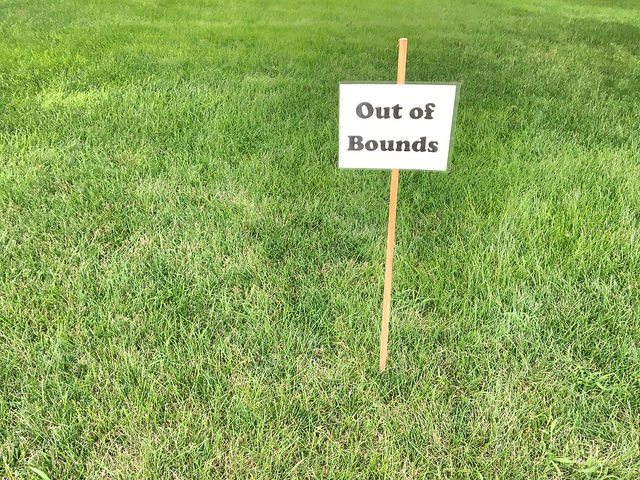
\includegraphics[width=0.6\textwidth]{figures/bounds.jpg}\\
		\hspace*{15pt}\hbox{\scriptsize Image By:\thinspace{\itshape David Mulder}}
		%https://www.flickr.com/photos/113026679@N03/43459273171
	\end{center}
\end{frame}

\begin{frame}
	\frametitle{A lower bound}
	\framesubtitle{Omega}
	\begin{definition}[Big-$\Omega$ (Omega)]
		A function $f(n)$ is $\Omega(g(n))$ iff there is a positive real constant $c$ and a positive integer $n_0$ such that for
		all $n \geq n_0$ it holds that $f(n) \geq c g(n)$. In other words:\\
		$\exists c \in \mathbb{R}, \exists n_0 \in \mathbb{N} (c > 0 \wedge n_0 \geq 1 \wedge (\forall n \in \mathbb{N} (n
		\geq n_0 \to f(n) \geq cg(n))))$.
	\end{definition}
	\pause
	\begin{questionblock}{What of it?}
		Assume that $f(n)$ is $O(g(n))$ what, if anything, can we now conclude?
		\begin{enumerate}[A.]
			\item $f(n)$ is $\Omega(g(n))$
			\item $g(n)$ is $O(f(n))$
			\item $g(n)$ is $\Omega(f(n))$
			\item None of the above.
			\item I don't know.
		\end{enumerate}
	\end{questionblock}
\end{frame}

\begin{frame}
	\frametitle{So what?}
	\begin{questionblock}{Why do we care?}
		What can we use big-$\Omega$ for?
	\end{questionblock}
	\pause
	\begin{answerblock}{Not much!}
		Very very little :) \\
		\pause
		Though occassionally we can prove things require e.g.\ $\Omega(n)$ steps, even if we do not know how to solve it
		exactly.\\
		\pause
		But if something is both $O(f(n))$ and $\Omega(f(n))$\dots
	\end{answerblock}
	\pause
	\begin{definition}[Big-$\Theta$ (Theta)]
		A function $f(n)$ is $\Theta(g(n))$ iff there are positive real constants $c_0, c_1$ and a positive integer $n_0$ such that for
		all $n \geq n_0$ it holds that $c_0 g(n) \leq f(n) \leq c_1 g(n)$. In other words:\\
		{\small
		$\exists c_0,c_1 \in \mathbb{R}, \exists n_0 \in \mathbb{N} (c_0> 0 \wedge c_1 > 0\wedge n_0 \geq 1 \wedge (\forall
		n \in \mathbb{N} (n \geq n_0 \to c_1 g(n) \leq f(n) \leq c_2 g(n))))$.
	}
	\end{definition}
\end{frame}

\begin{frame}
	\vspace{-10pt}
	\begin{overlayarea}{\textwidth}{\textheight}
			\begin{questionblock}{Why do we care about this?}
				So is big-$\Theta$ any use?
			\end{questionblock}
			\pause
	\vspace{-5pt}
			\begin{answerblock}{Yes!}
				It is basically the ``tight upper bound'' we discussed yesterday.
			\end{answerblock}
			\pause
	\vspace{-5pt}
		\only<-5>{
			\begin{columns}
				\column{0.455\textwidth}
				\lstinputlisting{code/big-oh-example.py}
				\pause	
				\column{0.455\textwidth}
				\alt<5>{
					\begin{answerblock}{Run time}
						The run time is described as $T(n) = c_0 + c_1n + c_2n^2$, where
						\begin{itemize}
							\item $c_0$ is for lines 2, 5, and 9.
							\item $c_1n$ is for the range in line 3.
							\item $c_2n^2$ is for lines 4, 5, and 8.
						\end{itemize}
						Thus $T(n)$ is $\Theta(n^2)$.
					\end{answerblock}
					}{
					\begin{questionblock}{So\dots}
						What is a tight bound on the run time of \texttt{maya}?
						\begin{enumerate}[A.]
						\small
							\item $\Theta(1)$
							\item $\Theta(n)$
							\item $\Theta(n^2)$
							\item $\Theta(n^3)$
							\item I don't know.
						\end{enumerate}
					\end{questionblock}
				}
			\end{columns}
		}
		\only<6>{
				\begin{alertblock}{Despite all that...}
					We still often \textit{just} ask for ``a tight upper bound'' and will accept a big-Oh.
				\end{alertblock}	
		}
	\end{overlayarea}
\end{frame}

